\chapter{Literature review}
\label{literature}

\section{Differential Analysis of Languages}

Language is a system that consists of the development, acquisition, maintenance and use of complex systems of communication, particularly the human ability to do so; and a language is any specific example of such a system. Estimates of the number of human languages in the world vary between 5,000 and 7,000. Languages as communication tools are different in many ways. Recall that when you first learn a second language (L2), the alphabet or words in that language looks so strange, especially for those languages using different sets of characters (for example Chinese and English). You may regard those words as a sequence of graphs without any meanings. Also, when you first listen to a sentence in the L2 or two people talking in L2, the sound waves are just noise to you. However, you are still aware that those sentences (either in text or sound format) are conveying specific information in a different way from your own language. How are languages different; where do those differences come from?

Language (or linguistic) typology is the science that studies ``similarities and differences among languages that do not stem from shared genetic relationship, language contact, or shared environmental conditions'' \citep{moravcsik_2012}. The goal of language typology is to describe and explain the common properties and structural diversity of the world's languages and how those properties generalize in cross-linguistic case \citep{bickel2001typology}. This discipline includes several subfields, depending on the ways languages are grouped into same class. An introductory categorization is provided by \cite{moravcsik2012introducing}:

\begin{enumerate}
\item Lexical typology: deals with characteristic ways in which language packages semantic material into words. For example, English uses different words for ``foot''/``leg'' and ``finger''/``toe'' while languages like Japanese and Russian use one word to represent ``foot''/``leg'' (``ashi'' in Japanese and ``noga'' in Russian) and ``finger''/``toe'' (``yubi'' in Japanese and ``palec'' in Russian).
\item Syntactic typology: deals with characteristic ways in which language packages words into sentences syntactically. For example, according to subject-verb-object positioning, languages can be grouped into different sets: SOV (such as French, German, Spanish and Chinese), SVO (such as English and Chinese) and so on, where the abbreviation represents the order of subject(S), verb(V) and object(O).
\item Morphological typology: deals with characteristics ways in which language forms words by combining morphemes. For example, morphological typology categorize languages into analytic languages and synthetic languages. Analytic languages, including Chinese and Vietnamese, contain very little inflection (inflection refers to ``the modification of a word to express different grammatical categories such as tense, case, voice, aspect, person, number, gender, and mood''), instead relying on features like word order and auxiliary words to convey meaning while synthetic languages, including most Indo-European languages, form words by affixing a given number of dependent morphemes to a root morpheme and word order is less important for synthetic languages.
\item Phonological typology: dealing with characteristics ways in which sounds are distributed across languages and phonological phenomena such as phoneme inventories, syllable structure, phonological alternations, stress/tone/intonation, prosodic morphology and so on. For example, in terms of consonant-vowel ratio, English is relatively low and Russian is relatively high. In terms of syllable structure, English is relatively complex while Mandarin is relatively simple \citep{wals}.
\end{enumerate}

As introduced in Chapter \ref{introduction}, the current study focuses on phonological patterns of L1 and L2 and how they affect the phonological patterns of accented speech. This section introduces the phonological difference among different languages and will ignore those non-phonological differences. There are several data sources for language typology: UCLA Phonological Segment Inventory Database \citep{maddieson1992ucla}, Word Atlas of Language Structures (WALS) \citep{wals}, URIEL Typological Database \citep{littel2016uriel}, PHOIBLE \citep{phoible}, to name a few. Different databases contain different data sources and language samples. Here, the features provided by WALS are used to illustrate the phonological difference among several languages for the reason that WALS provides simple ways to visualize and download the data.

\begin{figure}[h]
\centering
\captionsetup{justification=centering}
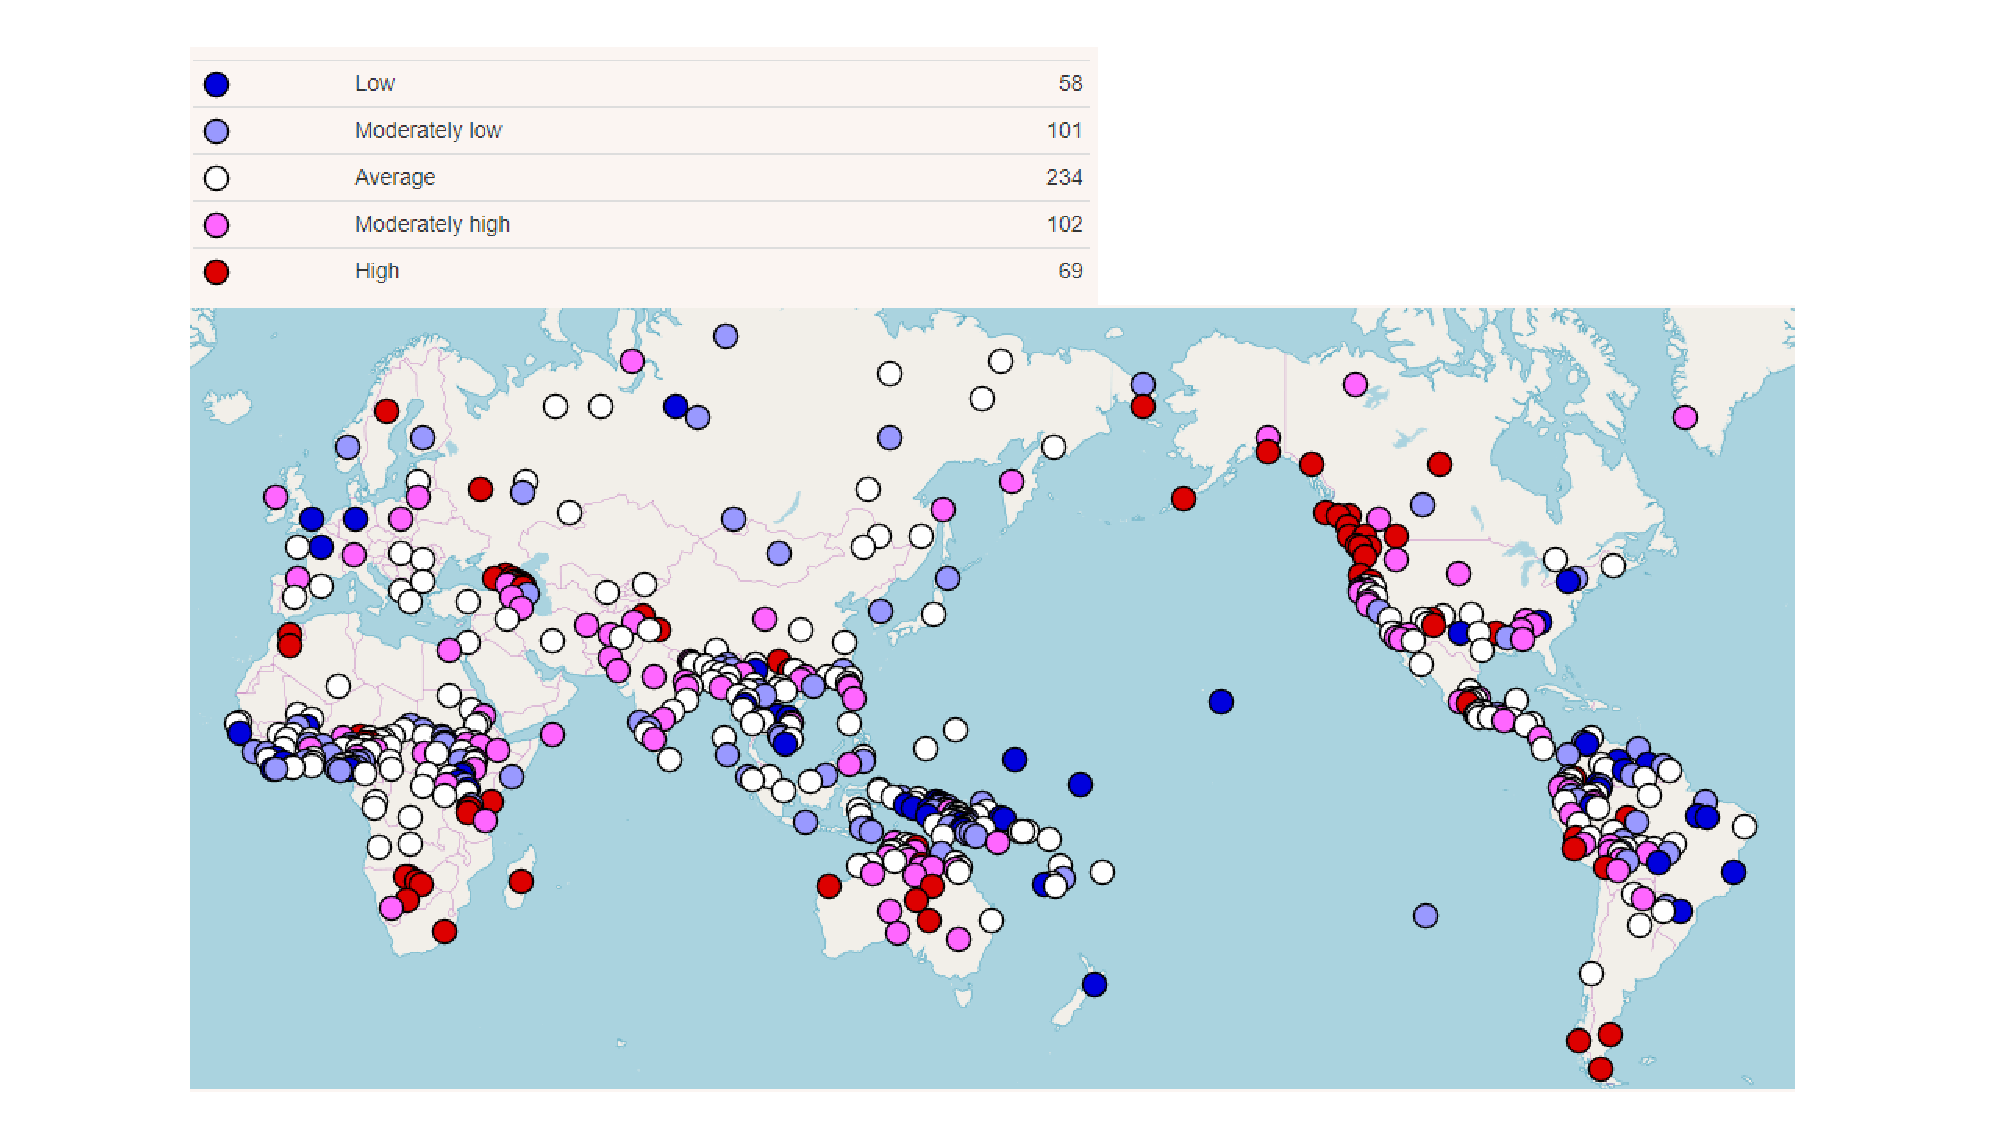
\includegraphics[width = 0.8\linewidth]{figures/WALS_example.pdf}
\caption{Consonant-vowel ratios across sampled languages by WALS. Different colors represent different levels of consonant-vowel ratios: blue for low level, light blue for moderately low level, white for average level, magenta for moderately high level and red for high level.}
\label{fig:wals_example}
\end{figure}

First, in figure \ref{fig:wals_example}, the consonant-vowel ratio illustrates how phonological patterns are different across world's languages. Higher ratio means there are more consonants and fewer vowels in that language, while lower ratio means the opposite. Take some commonly used languages as examples: English, German and French all have low ratios; Spanish, Persian and Mandarin have average ratios; Russian has a high ratio.

\begin{table}[]
\centering
\caption{19 language phonological features summarized by WALS. The last column indicates whether the feature is phonetic or rhythmic feature. For detailed description of each feature, refer to \cite{wals}}
\label{table: wals_feature}
\begin{tabular}{|c|c|}
\hline
Feature name & Phonetic or Rhythmic \\ \hline
Consonant Inventories & Phonetic \\ \hline
Vowel Quality Inventories & Phonetic \\ \hline
Consonant-Vowel Ratio & Rhythmic\tablefootnote{Although Consonant-Vowel Ratio looks like a phonetic feature because it is the ratio of the number of consonants and vowels, most studies regard it as a rhythmic feature \citep{gil1986prosodic}.} \\ \hline
Voicing in Plosives and Fricatives & Phonetic \\ \hline
Voicing and Gaps in Plosive Systems & Phonetic \\ \hline
Uvular Consonants & Phonetic \\ \hline
Glottalized Consonants & Phonetic \\ \hline
Lateral Consonants & Phonetic \\ \hline
The Velar Nasal & Phonetic \\ \hline
Vowel Nasalization & Phonetic \\ \hline
Front Rounded Vowels & Phonetic \\ \hline
Syllable Structure & Rhythmic \\ \hline
Tone & Rhythmic \\ \hline
Fixed Stress Locations & Rhythmic \\ \hline
Weight-Sensitive Stress & Rhythmic \\ \hline
Weight Factors in Weight-Sensitive Stress System & Rhythmic \\ \hline
Rhythm Types & Rhythmic \\ \hline
Absence of Common Consonants & Phonetic \\ \hline
Presence of Uncommon Consonants & Phonetic \\ \hline
\end{tabular}
\end{table}

Next, it is clear to do differential analysis of different languages with phonological patterns and to illustrate the distance among different languages on phonological feature space. To achieve this, several phonological features pre-summarized by WALS are selected. Based on whether there definitions are segmental or supra-segmental, those features are categorized into phonetic features and rhythmic features. Two groups of features represent language phonological patterns on phonetic space and rhythm space respectively. Table \ref{table: wals_feature} includes those features' names and indicates whether each feature is phonetic or rhythmic\footnote{Downloadable from \url{https://cdstar.shh.mpg.de/bitstreams/EAEA0-7269-77E5-3E10-0/wals_language.csv.zip}}. WALS assigns feature values to languages based on the structural properties of languages that describe one aspect of cross-linguistic diversity. For example, the feature ``Rhythm Types'' can take five values: Trochaic (left-hand syllable in the foot is strong), Iambic (right-hand syllable in the foot is strong), Dual (system has both trochaic and iambic feet), Undetermined (no clear foot type) and Absent (no rhythmic stress). Those feature values are stored as a number, usually starting from 1, to represent each category they belong to. To visualize those languages on a 2-dimensional space, the numeric values of each feature are employed. If one feature is not applicable to a language, 0 is used instead. As a result, each language will have a 19-dimensional feature vector representing values of those features in table \ref{table: wals_feature}. Each feature vector is also split into phonetic and rhythmic feature vectors. Since each feature actually indicates a category, to make sure the distances among different categories are the same, one-hot encoding converts the integer feature value to a vector consisting of 0s and 1s. The length of the encoded vector equals to the number of categories that feature can be. For example, the ``Rhythm Types'' feature has 5 categories. Then, a number of 3 will be encoded as ``00010''. Multidimensional scaling (MDS), which seeks a low-dimensional representation of those feature vectors in which the distances respect well the distances in the original high-dimensional space, is employed to illustrate the 2-dimensional representation of each language in all phonological feature space (as shown in figure \ref{fig:all_mds}), phonetic feature only space (as shown in figure \ref{fig:phonetic_mds}) and rhythmic feature only space (as shown in \ref{fig:rhythmic_mds}) with the encoded language features.

\begin{figure}
\centering
\minipage{0.55\textwidth}
  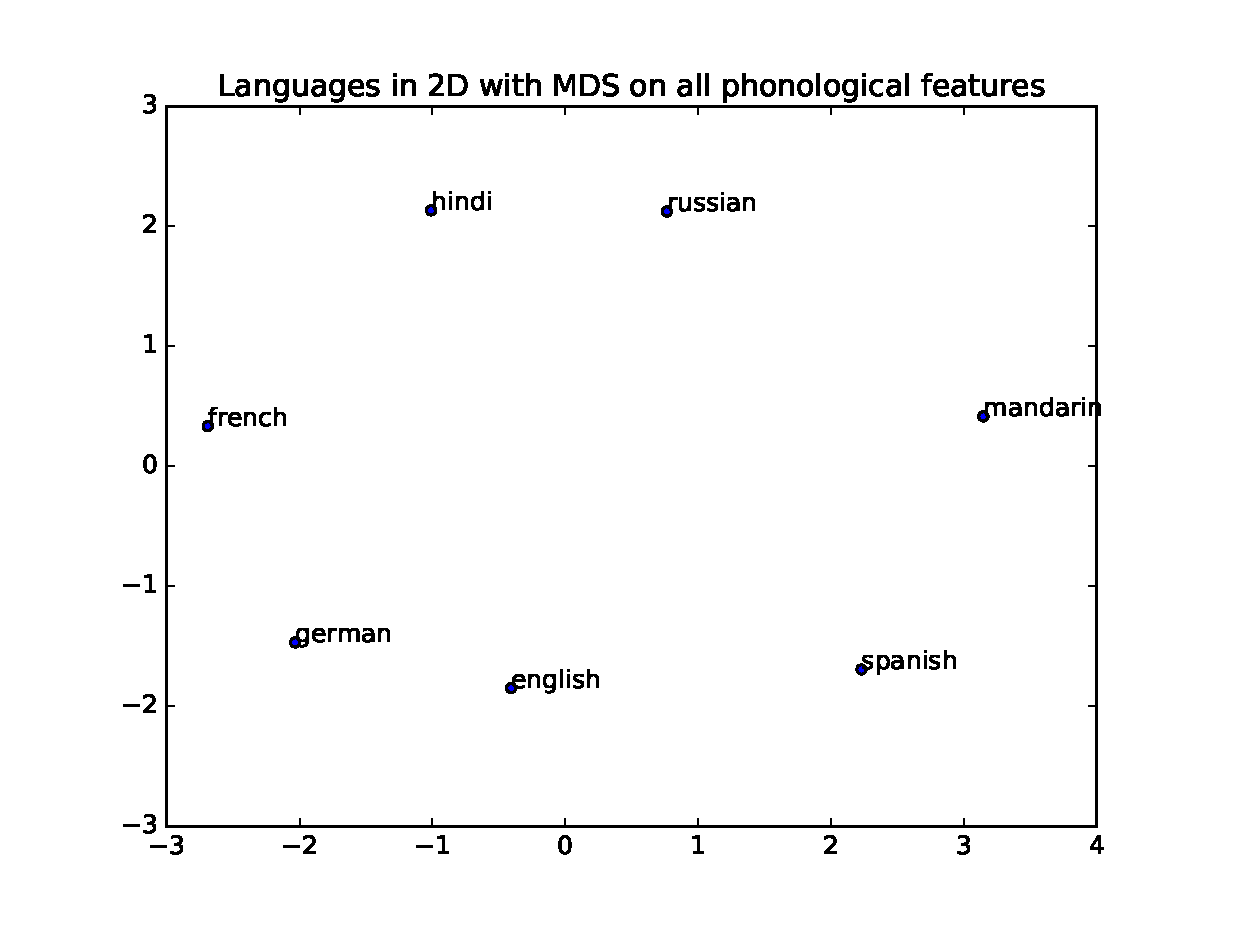
\includegraphics[width=\linewidth]{figures/all_MDS.eps}
  \caption{2D visualization of all features with MDS.}\label{fig:all_mds}
\endminipage\hfill
\\
\minipage{0.55\textwidth}
  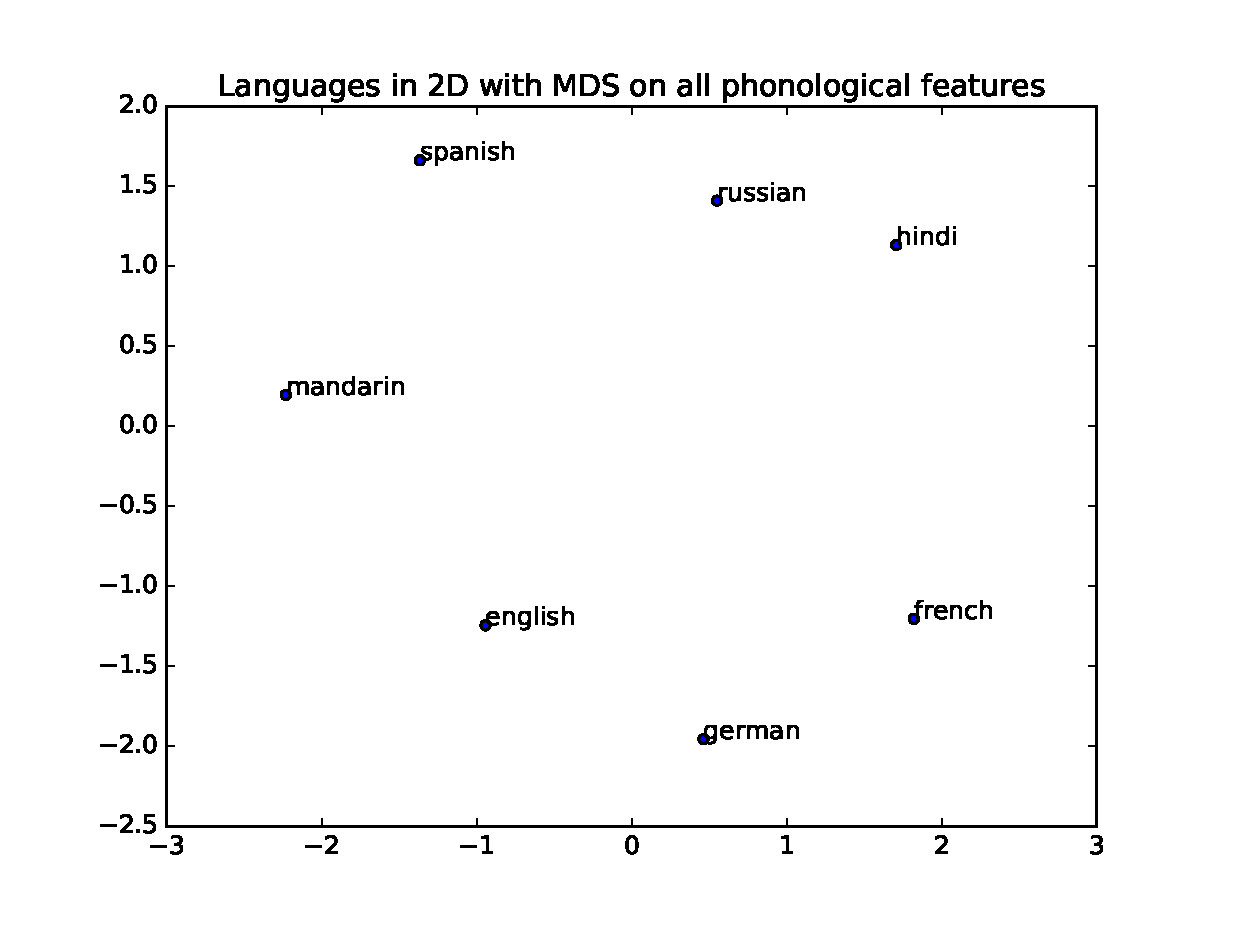
\includegraphics[width=\linewidth]{figures/phono_MDS_wals.eps}
  \caption{2D visualization of phonetic only features with MDS.}\label{fig:phonetic_mds}
\endminipage\hfill
\\
\minipage{0.55\textwidth}%
  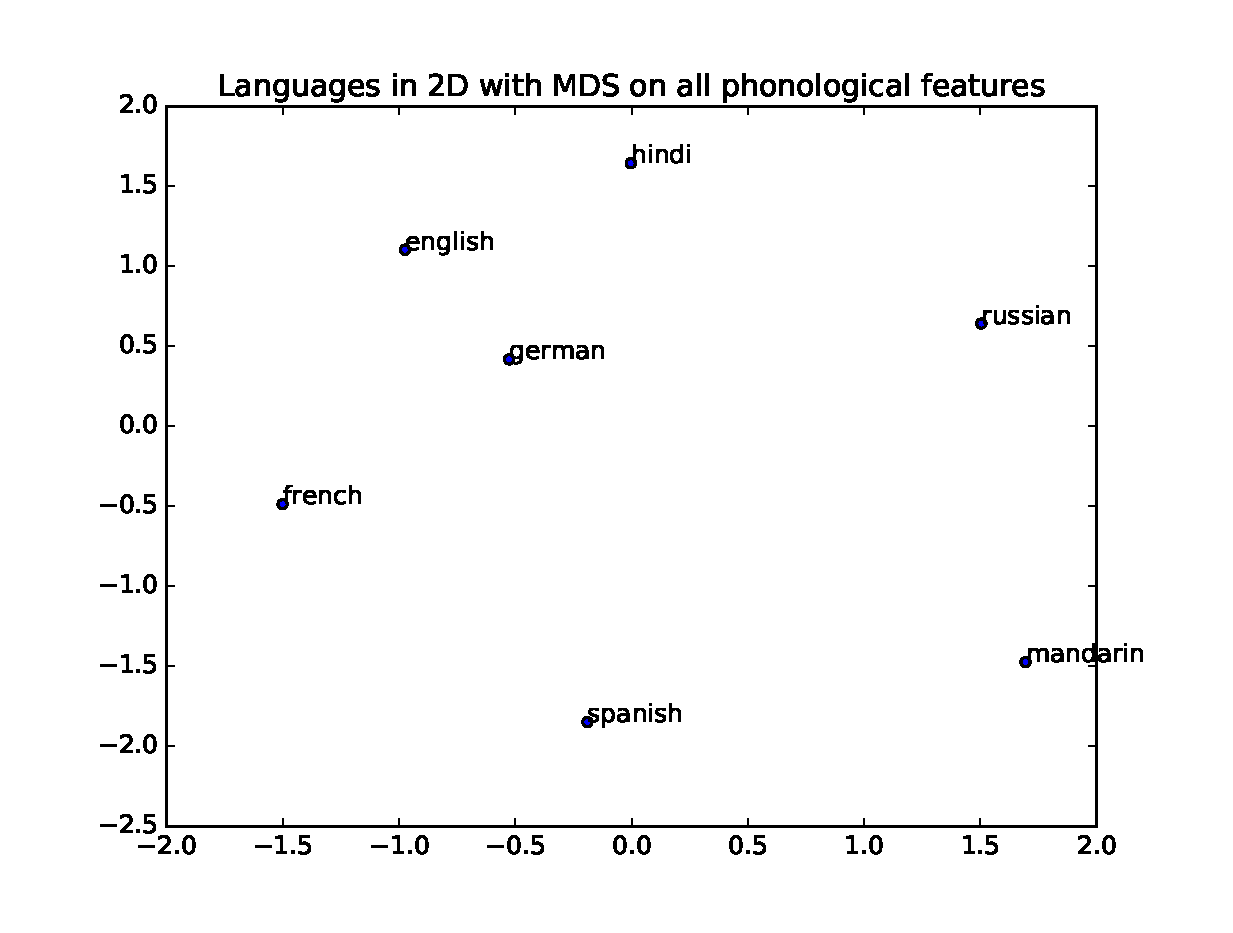
\includegraphics[width=\linewidth]{figures/rhythmic_MDS.eps}
  \caption{2D visualization of rhythmic only features with MDS.}\label{fig:rhythmic_mds}
\endminipage
\end{figure}

Along with the 2-dimensional visualization, normalized pair-wise distance matrices are also shown in table \ref{table:conf_all} for all features, table \ref{table:conf_phonetic} for phonetic features and table \ref{table:conf_rhythmic} for rhythmic features. The pairwise distance between two languages is calculated as follows: count the number of different values for corresponding dimensions of the feature vectors of two languages without one-hot encoding. This will result in a $N \times N$ matrix where N is the number of languages; normalize the matrix by the maximum value in the matrix. The feature visualization and normalized pair-wise distance matrices suggest that English, German and French are relatively close to each other on all three feature spaces while other languages are relatively far from those three languages. If English is regarded as L2, German is closest to English on the space specified by all features. Furthermore, German is closer to English on rhythmic space than phonetic space. So is French. However, Mandarin and Spanish are closer to English on phonetic space than rhythmic space. One important question this study wants to investigate is whether those L1 to L2 distance patterns will manifest in the accented speech perception: how the relative importance of segmental features and supra-segmental features relates to the distance to L2 on phonetic and rhythmic spaces.

\begin{table}[t]
\centering
\caption{Normalized pairwise distance on all features space.}
\label{table:conf_all}
\resizebox{0.55\columnwidth}{!}{%
\begin{tabular}{|c|c|c|c|c|c|c|c|}
\hline
 & German & Spanish & French & Russian & Hindi & English & Mandarin \\ \hline
German & 0 & 0.92 & 0.33 & 0.67 & 0.67 & 0.33 & 0.83 \\ \hline
Spanish &  & 0 & 0.83 & 0.67 & 0.75 & 0.67 & 0.50 \\ \hline
French &  &  & 0 & 0.67 & 0.58 & 0.58 & 1.00 \\ \hline
Russian &  &  &  & 0 & 0.42 & 0.58 & 0.75 \\ \hline
Hindi &  &  &  &  & 0 & 0.50 & 0.92 \\ \hline
English &  &  &  &  &  & 0 & 0.83 \\ \hline
Mandarin &  &  &  &  &  &  & 0 \\ \hline
\end{tabular}}
\end{table}

\begin{table}[t]
\centering
\caption{Normalized pairwise distance on phonetic features only space.}
\label{table:conf_phonetic}
\resizebox{0.55\columnwidth}{!}{%
\begin{tabular}{|c|c|c|c|c|c|c|c|}
\hline
 & German & Spanish & French & Russian & Hindi & English & Mandarin \\ \hline
German & 0 & 1.00 & 0.29 & 0.71 & 0.86 & 0.43 & 0.71 \\ \hline
Spanish &  & 0 & 1.00 & 0.57 & 0.71 & 0.57 & 0.43 \\ \hline
French &  &  & 0 & 0.71 & 0.57 & 0.71 & 1.00 \\ \hline
Russian &  &  &  & 0 & 0.29 & 0.57 & 0.71 \\ \hline
Hindi &  &  &  &  & 0 & 0.71 & 0.86 \\ \hline
English &  &  &  &  &  & 0 & 0.71 \\ \hline
Mandarin &  &  &  &  &  &  & 0 \\ \hline
\end{tabular}}
\end{table}

\begin{table}[t]
\centering
\caption{Normalized pairwise distance on rhythmic features only space.}
\label{table:conf_rhythmic}
\resizebox{0.55\columnwidth}{!}{%
\begin{tabular}{|c|c|c|c|c|c|c|c|}
\hline
 & German & Spanish & French & Russian & Hindi & English & Mandarin \\ \hline
German & 0 & 0.80 & 0.40 & 0.60 & 0.40 & 0.20 & 1.00 \\ \hline
Spanish &  & 0 & 0.60 & 0.80 & 0.80 & 0.80 & 0.60 \\ \hline
French &  &  & 0 & 0.60 & 0.60 & 0.40 & 1.00 \\ \hline
Russian &  &  &  & 0 & 0.60 & 0.60 & 0.80 \\ \hline
Hindi &  &  &  &  & 0 & 0.20 & 1.00 \\ \hline
English &  &  &  &  &  & 0 & 1.00 \\ \hline
Mandarin &  &  &  &  &  &  & 0 \\ \hline
\end{tabular}}
\end{table}

The previous features are summarized by linguistics on a high systematic level. How do those features manifest themselves in the acoustic recordings of different languages? How do the languages' differences manifest themselves in the key parameters of acoustic speech signal, including intensity, pitch, formants, envelop and so on? Several studies have investigated this. An early study \citep{parmenter1933experimental} compared the acoustic characteristics between English and French reading speech, and showed that pitch is more important as an element of accent than intensity for French speech, while intensity is more important for English speech. Also, French speech has more pitch variation than English. Studies by \cite{jongman1989acoustic,bradlow1995comparative,al2005does} investigated the relationship between vowel inventories and vowel space (defined as the two-dimensional area bounded by lines connecting first and second formant frequency coordinates of vowels \citep{fant1973speech}), and concluded that vowel space depends on the size of vowel inventory: the larger the inventory, the bigger the acoustic space. The work by \cite{wagner2003voice} showed that predominant factors in voice quality are different across different languages. In terms of speech rhythm, an influential study by \cite{ramus1999correlates} investigated the representation of linguistic speech rhythm in acoustic speech signal. Several acoustic measurements for speech rhythm are proposed to discriminate the rhythm classes of different languages. Those measurements include the percentage of vocalic segment in an utterance ($\%V$), the standard deviation of consonant intervals ($\Delta C$) and the standard deviation of vowel intervals ($\Delta V$). Figure \ref{fig:rhythm_lang} is taken from \citep{ramus1999correlates} to show how $\%V$ and $\Delta C$ can discriminate languages. Based on this study, other measurements like variational coefficient of consonant/vowel intervals \citep{dellwo2006rhythm} and pairwise variability index (PVI) of consonant/vowel intervals \citep{grabe2002durational} are also proposed. Studies that correlate those linguistically summarized phonological language features with acoustic measurements lay the foundation of the methodology used in this study.

\begin{figure}
\centering
\captionsetup{justification=centering}
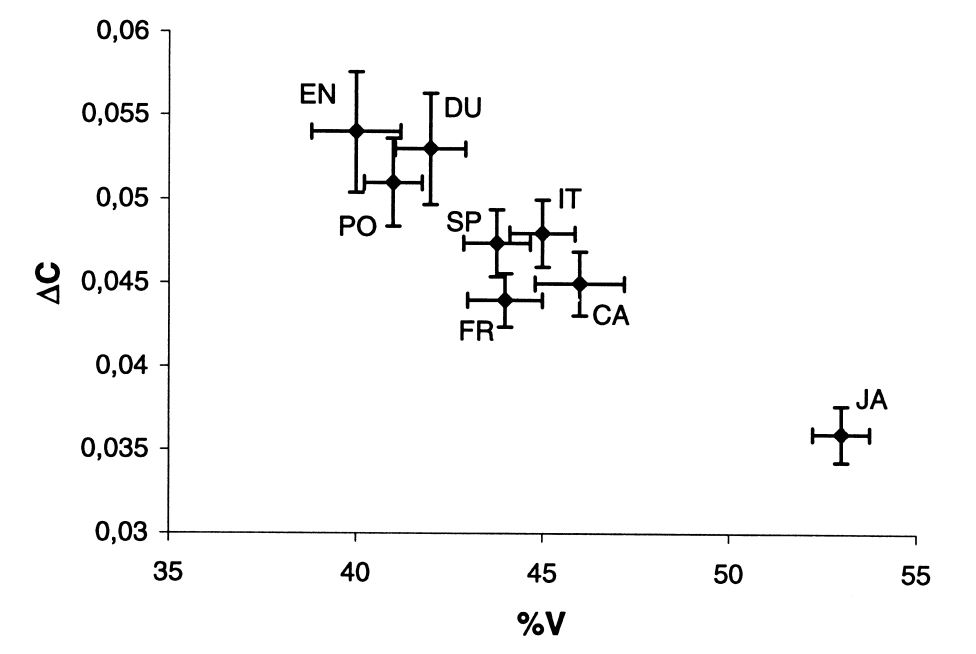
\includegraphics[width = 0.8\linewidth]{figures/ramus_paper.JPG}
\caption{Distribution of languages over the ($\%V$, $\Delta C$) plane. EN: English, PO: Polish, DU: Dutch, SP: Spanish, IT: Italian, FR: French, CA: Catalan, JA: Japanese. Taken from \citep{ramus1999correlates}}
\label{fig:rhythm_lang}
\end{figure}

\section{L2 learning theories}

In literature, there is a huge body of research on the L1 acquisition: how a child acquires a complicated linguistic system including different levels of information without explicit guidance. As summarized by \cite{chang2010first}, those studies both investigated the effect of an innately endowed Universal Grammar, and the effect of the timely input on L1 acquisition. A similar research track has been borrowed to study the L2 learning theories: investigating both the influence of already built linguistic system (L1) and some universal effects that are independent of the already built linguistic system. It has been shown that while moving toward to the target L2 linguistic system, L2 learners usually show trackable difference from the implementation of native L2 speakers, which is attributed to the influence of the learner's L1. In terms of phonology, this is where the perceived foreign accent comes from. Considering L1 interference mechanism, i.e., the phonological knowledge transfer from L1 to L2, are focused by the majority of the literature and is more related to the current study, in this chapter research body on phonetic acquisition will be reviewed. Specifically, some well-established L2 learning theories focusing on the accented phoneme production will be introduced first. Then, studies on speech prosody acquisition in L2 learning will be covered. The last subsection will focus on the role of L1 in L2 learning and elaborate more on the L1's interference in L2 learning.

\subsection{Phonetic acquisition}

There have been studies trying to explain the origin of the foreign accent in producing L2 phonemes. The critical period hypothesis from L1 acquisition was extended to L2 acquisition, positing that there is a critical age or period after which L2 speech production could not be native-like because of the neurological maturation \citep{long1990maturational}. Other studies assume the failure to acquire native-like production of L2 is caused by factors like inaccurate perception of L2 sounds, inadequate phonetic input, insufficient motivation, psychological reasons and incorrect L2 learning habit because of incorrect instructions \citep{flege1988production}. Although all these observations partly show evidence of the origin of the foreign accent, they fail to explain the L2 learning process in a systematic way, and how L2 learning is different from L1 acquisition. Nonetheless, there is consensus achieved by the community that the earlier one starts to learn a L2, the better\footnote{There are still some outliers found by researchers, for example it was reported that both early L2 learners still failed to achieve native-like production while late L2 learners did \citep{flege1995second}}.

Developed by \cite{flege1995second}, the speech learning model (SLM) is the most influential study in L2 speech learning literature. Different from the critical period hypothesis, SLM assumes that the phonetic systems used in the production and perception of vowels and consonants is active during the whole life span. It functions like a dynamic system that can encode all phonetic input. As mentioned in \citep{flege1995second}, ``the phonetic systems reorganize in response to sounds encountered in an L2 through the addition of new phonetic categories, or through the modification of old ones''. L1 and L2 phonetic categories exist in a shared system, and there is motivation to keep them distinct from each other. This indicates that the formation of the phonetic system of accented speech is based on the L2 learner's already-established L1 phonetic system. To explain this age-related L2 learning process, SLM has 4 postulates and 6 hypotheses. The 4 postulates \citep{flege1995second} are:

\begin{enumerate}
\item The mechanisms and processes used in learning the L1 sound system, including category formation, remain intact over the life span, and can be applied to L2 learning.
\item Language-specific aspects of speech sounds are specified in long-term memory representations called phonetic categories.
\item Phonetic categories established in childhood for L1 sounds evolve over the life span to reflect the properties of all L1 or L2 phones identified as a realization of each category.
\item Bilinguals strive to maintain contrast between L1 and L2 phonetic categories, which exist in a common phonological space.
\end{enumerate}

The 6 hypotheses are based on those 4 postulates and on evidence from data analysis in previous studies on speech production of l2 learners. Next, each hypothesis together with evidence and predicts will be introduced (most of them can be found in the review paper by \cite{flege1995second}).

\textbf{Hypothesis 1:} sounds in the L1 and L2 are related perceptually to one another at a position-sensitive allophonic level, rater than at a more abstract phonemic level. L2 learners will perceive positional allophones in the L2 to the most similar positionally defined allophone in the L1. Studies have shown that it is easier for L2 learners to produce and perceive certain allophones of English phonemes than others. Native Japanese speakers are taken as example. It is hard for native Japanese speakers producing and perceiving English /\textipa{l}/ and /\textipa{r}/, because in Japanese, there is only one liquid while English has two. Thus, the contrast between /\textipa{l}/ and /\textipa{r}/ is difficult to attain. However, it has been found that the production accuracy of these two liquids depends on phonological environments. In \citep{strange1992learning}, the authors showed that native Japanese learners of English characteristically perceive and produce English liquids more accurately in word-final than word-initial position. They attributed this to that the acoustic difference between English /\textipa{l}/and /\textipa{r}/ is more robust in final than initial position \citep{sheldon1982acquisition}. This indicates the position-sensitive relationship between L1 and L2 sounds in allpphonic level.

\textbf{Hypothesis 2:} a new phonetic category can be established for an L2 sound that differs phonetically from the closest L1 sound if bilinguals discern at least some of the phonetic differences between the L1 and L2 sounds. The likelihood of the formation of a new phonetic category increases with the dissimilarity between an L2 sound and the closet L1 sound. Several studies have shown that when a novel phoneme (not exists in L1 or very different from L1 phonemes) is encountered, L2 learners can usually produce it accurately. In \citep{flege1987production}, the authors found that native English speakers can produce the French vowel /\textipa{y}/, a vowel that does not exist in English, relatively accurately compared to native French speakers. \cite{flege1997english} further showed that native Dutch speakers can produce the English vowel /\textipa{\ae}/ accurately, and similar results were found in another study on German speakers \citep{flege1997perception}. Those findings suggest that if the phonetic differences between the L2 sound to the closet L1 sound are obvious, the production of the L2 sound can be produced accurately because a new phonetic category is employed to produce the sound.

\begin{figure}
\centering
\captionsetup{justification=centering}
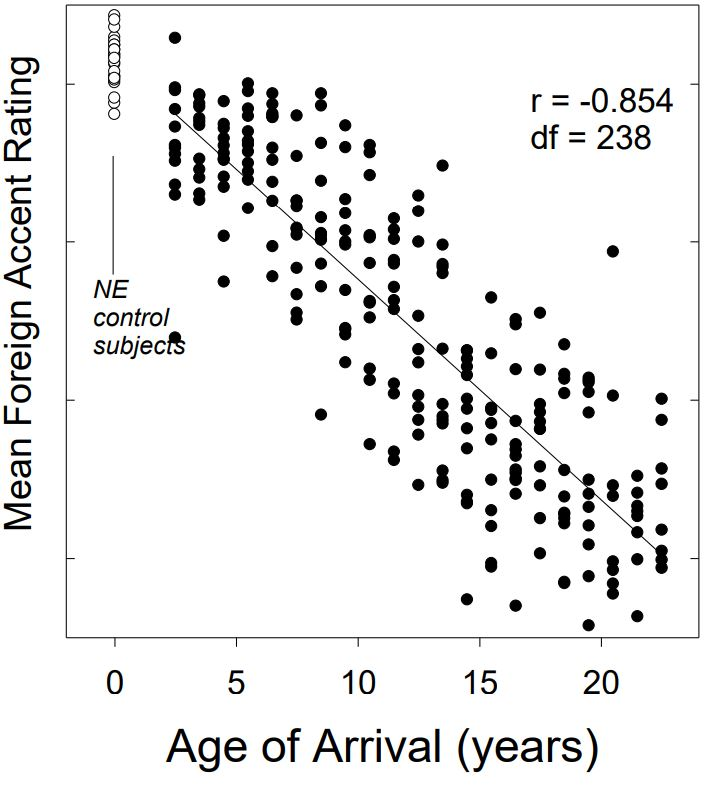
\includegraphics[width = 0.8\linewidth]{figures/accentedness_AOA.JPG}
\caption{The mean foreign accent ratings (Y-axis) of English sentences spoken by native Korean immigrants to US. X-axis represents the age of arrival. Taken from \citep{flege1999native}.}
\label{fig:accent_example}
\end{figure}

\textbf{Hypothesis 3:} The likelihood of phonetic differences between L1 and L2 sounds, and between L2 sounds that are noncontrastive in the L1, being discerned decreases as the age of learning increases. For example, the study in \citep{butcher1978influence} showed that the perceived distance between /\textipa{ae}/ in English and /\textepsilon/ in German is greater for German children than adults. \cite{weiher1975lautwahrnehmung} also showed that German adults, but not children, have difficulty discriminating /\textipa{ae}/ in English and /\textepsilon/. Based on this hypothesis, it can be predicted that, with the increasing of the age of learning, more sounds in L2 will be inaccurately produced. Thus, a linear relationship between perceived accentedness and age of learning is shown in figure \ref{fig:accent_example}, in contrast to the sharp discontinuity in the L2 pronunciation ability suggested by the critical period hypothesis.

\textbf{Hypothesis 4:} Category formation for an L2 sound may be blocked by the mechanism of equivalence classification. When the block occurs, speakers tend to use a single phonetic category to process perceptually similar L1 and L2 sounds, resulting in inaccurate production of L2 sounds. The study by \cite{flege1987production} showed that French learners who are native American English speakers produce the French phoneme /\textipa{u}/ with second formant ($F_2$) values higher than native French speakers, which is influenced by the high-$F_2$ /\textipa{u}/ in English. \cite{chang2008phonetic} also reported that native American English speakers also produce Mandarin phoneme /\textipa{u}/ with higher $F_2$. \cite{flege1987production} also showed that native English speakers produce French voiceless stops with too long voice onset times (VOTs), under influence from the long-lag VOT of English voiceless stops.

\textbf{Hypothesis 5:} The phonetic category established for L2 sounds by a bilingual may differ from a monolingual's if: 1) the bilingual's category deviates from an L2 category to maintain phonetic contrast between categories in a common L1-L2 phonological space; or 2) the bilingual's representation is based on different features, or feature weights, than a monolingual's. The evidence can be found in the study by \cite{munro1993productions}, where the authors showed that even experienced L2 English speakers, who are native Arabic speakers, produce vowels that are considered to have accent. According to the study, the accentedness was due to non-native production of duration differences between tense and lax English vowels. They suggest that in this case, the L2 tense and lax categories might have been interpreted as long and short categories, which exist in Arabic. The evidence of the second point is shown in the study by \cite{munro1996effects}. This study showed that English learners with Italian as the native language can not produce accurate phoneme /\textrhookschwa/, although those learners started to speak English at ten years of age and were rated to have a very mild foreign accent. The authors considered the reason to be related to the retroflex feature that is used to discriminate from other English vowels, but the feature does not exist in Italian.

\textbf{Hypothesis 6:} The production of a sound eventually corresponds to the properties represented in its phonetic category representation. This hypothesis can be regarded as the result of hypothesis 2, 4 and 5, stating the L2 sound will eventually be produced as specified in phonetic category representation. If the presentation matches the category for native L2 speakers, then the L2 sound can be produced accurately; if new phonetic category for L2 sounds is not formed or different from monolingual's, there will be inaccurate pronunciation.

To summarize, SLM claims that the age of learning has significant influence on second language learning: this can be seen from those hypotheses that the age of learning directly influences the formation of phonetic categories to produce L2 sounds. Also, pre-established L1 phonetic categories will affect the way L2 sounds are perceived, and thus will also influence the formation of phonetic categories. If sounds in L2 are too close to sounds in l1, then equivalence classification will use the same phonetic category to produce the similar sounds, resulting in perceivable inaccurate pronunciation for L2 native speakers. Sometimes, phonetic categories built for novel L2 sounds can still be different from native's due to the dissimilation occurs between L1 and L2 phonetic categories to maintain phonetic contrast between categories in a common L1-L2 phonological space. This study mainly reviews the SLM model because it is highly related with the current study in a way that it directly explains how L2 learners develop inaccurate pronunciation of L2. Another wll-known model, the Perception Assimilation Model (PAM) \citep{best1995chapter,best2007nonnative} mainly deals with how a listener perceptually assimilates contrastive information between his L1 and a new language he does not know or just begins to learn. However, this study mainly deals with speakers who are not beginners of L2 learning. Thus, the literature on PAM is not reviewed here.

SLM mainly deals with phonetic acquisition, i.e. the segmental accuracy of L2 production. However, several studies have shown that inaccurate supra-segmental productions can also result in perceivable foreign accent \citep{rognoni2013testing,winters2013perceived}. In the next subsection, speech prosody acquisition in the literature will be reviewed to reveal the mechanism L2 learners use to achieve native-like productions of speech prosody.



\subsection{Prosody acquisition}

In the previous subsection, fundamental studies on L2 learning are reviewed. Those studies mainly focus on the phonetic part in terms of the whole phonological system. Although the study by \cite{munro1993productions} investigated the durations of tense and lax English vowels produced by native Arabic speakers and durations of vowels are related to speech prosody \citep{ramus1999correlates}, most analysis in these studies only dealt with pronunciation of specific phonemes; some even used isolated phonemes or words \citep{flege1987production}. Whether the theories proposed by these studies can be applied to prosodic inaccuracy of non-native L2 speech is still questionable \citep{rasier2007prosodic}. On the other hand, a review survey by \cite{gut2009non} showed that for all studies on L2 speech learning from 1969 to 2008, L2 intonation was only investigated in nine studies and L2 speech rhythm was only investigated in four studies \citep{mennen2004bi,altmann2006perception,rasier2007prosodic,lin2008interlanguage}. This indicates that the speech prosody in L2 speech is quite underexplored. This subsection will review literatures on acquisition of speech prosody acquisition during L2 learning.

The study by \cite{mennen2004bi} investigated how the non-native speakers of Greek whose L1 is Dutch realize the timing of a phonologically identical rise: nonfinal or prenuclear rises. This phonological property was realized differently by native Dutch and native Greek speakers: 1) at a different time: the peak in the rise appeared earlier in Dutch than in Greek. 2) The peak time in Dutch depends on the the phonological length of the vowel of accented syllable while Greek did not. By analyzing the timing patterns of the rise using five native Dutch speakers speaking Greek, the authors concluded that there existed a bi-directional interference in the realization of the rising accent: the L1 Dutch affected the realization in Greek and the L2 Greek also affected the realization in Dutch. The dissertation by \cite{altmann2006perception} studied the perception and production of advanced learners of English with different L1 backgrounds (Arabic, Chinese, French, Japanese, Korean, Spanish, Turkish) to investigate the effect of L1 stress properties on the L2 acquisition of primary word stress. The results showed that native speakers of L1s with predictable stress found it difficult to locate the stress in English although they were able to produce the correct stress patterns; native speakers of L1s without word-level stress or predictable stress performed well in stress perception but had difficulties in stress production. These results seem to contradict the SLM: good perception of stress patterns does not mean good production. \cite{rasier2007prosodic} reviewed the prosody acquisition of L1 learning and proposed a general framework to study the prosody transfer from L1 to L2 in L2 learning. The model was tested in a study of accent in L2 Dutch proposed by native French speakers and L2 French produced by native Dutch speakers. Their results showed that the difference between French and Dutch on accent placement influenced the acquisition process of accentuation. The ``Markedness'' proposed in \cite{eckman1977markedness} is an important factor in predicting and explaining learning difficulties in L2 prosody learning.

The previous studies mainly focus on stress and accent. The following introduced studies in this paragraph investigate the prosodic properties' acquisition in terms of duration and duration variability measurements, which have been shown to able to discriminate among languages within different rhythmic classes \cite{ramus1999correlates,grabe2002durational}. Those measurements include:

\begin{enumerate}
\item $\Delta V$: the standard deviation of vocalic intervals
\item $\Delta C$: the standard deviation of consonantal intervals
\item $\%V$: percentage of vocalic intervals in the sentence
\item $VarcoV$: the standard deviation of vocalic intervals divided by the mean vocalic interval duration and multiplied by 100
\item $VarcoC$: the standard deviation of consonantal intervals divided by the mean consonantal interval duration and multiplied by 100
\item $nPVI-V$: the normalized PVI for vocalic intervals
\item $rPVI-C$: the raw PVI for consonantal intervals
\end{enumerate}

One study \citep{stockmal2005measures} examined speech rhythm of the Latvian produced by native Russian learners. In their result, there was no clean increase in vocalic variability between experienced and low-level learners, despite the fact that Latvian is significantly less stress-timed than Russian. They concluded that even if the learner's L1 is stress-timed and has higher vocalic variability, at the early stage of acquisition the accented speech can still match the L2 in terms of lower vocalic variability. They also found that the consonantal duration variability increased significantly during L2 acquisition and attributed to the difficulties of consonants articulation. \cite{white2007calibrating} used all the seven rhythmic measurements, showing that those measurements were able to separate stress-timed English and Dutch and syllable-timed Spanish and French. They also applied the measurement to quantifying the influence of L1 on L2 rhythm acquisition when switching between stress-timed and syllable-timed. In an experiment consisting of native Spanish subjective speaking English and native English speakers speaking Spanish, it was found that the $VarcoV$, $nPVI-V$ and $rPVI-C$ were in the intermediate stage during the transfer from L1 to L2, indicating clearly the influence of L1 rhythm on l2. In the experiment consisting of native Dutch subjective speaking English and native English speakers speaking Dutch (both the two languages are stress-timed), it was found that there was no clear influence of L1. The authors believed that if L1 and L2 are already rhythmically similar, the L2 learners tend to make little accommodation and use their L1 rhythmic patterns. \cite{lin2008interlanguage} examined the accented English speech produced by native Mandarin speakers in terms of four measurements of speech rhythm: $\%V$, $\Delta C$, $rPVI-C$ and $nPVI-V$. With the reading and conversational recordings of 6 subjects, the authors showed that the value of $\%V$ of Mandarin accented English is in the middle of the value of native English speakers (lower) and native Mandarin speakers (higher). They explained that this indicated the L1 rhythm patterns had an effect on L2 rhythm patterns in terms of $\%V$. The average nPVI value was very close to native English speakers, and the authors attributed this to that those Mandarin subjects mastered the vocalic variability. However, the average values of the other two measurements are way higher than native English speakers. The authors believed it was because the consonantal duration patterns were much harder to acquire for Mandarin speakers when speaking English. Similar results were also reported by \cite{kawase2016influence} where the rhythmic acquisition of native Japanese (mora-timed) learners of English (stress-timed) was studied. \cite{li2014l2} conducted experiments on durational variation in L2 English productions by L1 Mandarin learners and L1 German learners and compared it to native control values in English. The results showed that the L1 groups followed comparable developmental paths in their acquisition of vocalic variability and accentual lengthening. However, the two L1 groups diverged in the proportion of vocalic materials in their L2 utterances and indicated L2 acquisition patterns that are consistent with direct transfer from the L1. Thus, they claimed that there was a multisystemic model of L2 rhythm acquisition. Both transferred L1 knowledge and universal effects independent of L1 played a role. \cite{ordin2015acquisition} did similar experiments to examine the differences in durational variability (several rhythmic measurements) between proficiency levels in L2 English spoken by French and German learners. They found that speech rhythm in L2 English learners in both groups developed from more syllable-timed toward more stress-timed patterns irrespective of the L1 had similar rhythmic patterns. However, they also showed that there were differences between the German and French groups: German learners achieved a degree of durational variability typical of the target language while French learners exhibited lower variability than native speakers.

Some recent studies investigated the relative importance of suprasegmental measurements to accentedness perception compared to segmental measurements. \cite{rognoni2013testing, winters2013perceived} transplanted the prosody measurements (F0 and duration) between native English speech and accented English speech in both directions to analyze the relative importance of segmental and suprasegmental features' contribution to accentedness perception. They both found that though prosodic features contributed to the perception of accentedness, segmental features were more important than suprasegmental features. The study by \cite{polyanskaya2016relative} applied the similar transplantation method to speaking rate and speech rhythm and concluded that speech rhythm contributed more to accentedness perception than speaking rate. A later study by \cite{van2017l1} further investigated the interplay of different rhythmic measurements including intonation, rhythm and speech rate. The authors found that while all measurements contributed to accentedness perception, intonation contributed the most for Dutch learners. However, all of these studies only did the transplantation on one foreign language (Italian, German, French or Spanish) and the contrastive information among different L1s was ignored. Another work by \cite{saito2016second} studied the relative contribution of segmental and supra-segmental to accentedness at different proficiency levels through regression analysis. Their subjects were Japanese who were learning English at different stages.

The prosody acquisition during L2 learning can be summarized as following:
\begin{enumerate}
\item Although there are evidences showing that some universal effects exist in prosody acquisition, most studies report the influence of the L1 on the prosody production of L2. This is similar to the phonetic acquisition.
\item Not all of the prosodic properties depend on the L1 during speech prosody acquisition, despite the fact that those properties can well discriminate between L1 and L2.
\item When the contrastive information between L1 and L2 can be well perceived, the prosody acquisition follow a path from L1 prosody features to L2 prosody features; when the contrastive information between L1 and L2 is not well perceived or the L1 and L2 prosodic patterns are very close, there is no clear sign of the influence of L1 prosodic patterns.
\end{enumerate}


\subsection{Role of L1 in L2 learning}

In the last two subsections, studies dealing with the phonological system acquisition during L2 learning are introduced. However, many studies only investigate one pair of L1 and L2: a one to one mapping, which can not reveal whether the difference of L1s can be projected to the accented L2 speech. Combining the acquisition of L2 in both segmental and supra-segmental perspective, it can be found that different L1s can result in different developments of L2 acquisition. A following question is how the segmental and supra-segmental production developments of L2 learners from different L1s are different. Since L1s have very different segmental and supra-segmental characteristics compared to L2, L2 learners from those L1s should undergo different procedures in both segmental and supra-segmental feature space, as in the findings by \cite{ordin2015acquisition}, although there exist some universal effects. In this subsection, a brief introduction of studies examining multiple L1s and one or multiple L2s are reviewed.
\cite{arslan1997study} calculated four temporal measurements: word-final stop closure duration, VOT, average voicing duration and word duration, across three L1 accents (German, Mandarin and Turkey) for a set of English words (``target'', ``teeth'', ``catch'', ``communication''), which include a stop consonant in the initial position. While word-final stop closure duration was found to be most discriminative among accents, various accents showed very different patterns in terms of the four measurements. English words with Mandarin accents are the most different from native produced words. German and Turkey speakers are relatively closer to native produced words compared to Mandarin. \cite{mccullough2013perceived} investigated the correlation between different segmental measurements in non-native speech and the perceived accentedness. Speakers from different L1 backgrounds (Hindi, Mandarin and Korean) were rated and analyzed based on their produced English speech. They showed that Hindi has the strongest accent compared to Mandarin and Korean speakers. Analysis of measurements including VOT, vowel quality (measured by F1 and F2 of vowel), vowel durations and F0 differences indicated that non-native speech produced by Hindi speakers showed clear difference compared to Mandarin and Korean speakers, while Mandarin and Korean speakers had similar patterns. For supra-segmental measurements, \cite{ramus1999correlates} studied the rhythmic properties across eight languages (English, Polish, Dutch, French, Spanish, Italian, Catalan and Japanese) and applied acoustical rhythmic measurements to language discrimination. They plotted these eight languages on a three dimensional rhythmic space consisting of 1) the proportion of vocal intervals within the sentence 2) the standard deviation of the duration of vocalic intervals within each sentence 3) the standard deviation of the duration of consonantal intervals within each sentence. The results indicated that there may be more information decided by speech rhythm rather than just the classification of stress-, syllable and mora-timed languages. Also, the difference among different L1s was very obvious. This study inspired the work by \cite{white2007calibrating} and \cite{lai2013applying}, where the authors applied similar acoustic analysis of the rhythm properties of both reading and spontaneous L2 speech. \cite{white2007calibrating} applied similar acoustical rhythmic measurements to quantifying the influence of L1 on L2 rhythm. They expected that speakers switching ``rhythm class (stress-timed or syllable timed)'' should show rhythm scores different from both their native and target languages. They found that the standard deviation of vocalic interval duration divided by the mean vocalic interval duration offered the most discriminative analysis of L1, L2 and L1 accented L2, which suggests L1 accented L2 is like an intermediate stage during the transfer from L1 to L2, and speakers with different L1 backgrounds show differences in their accented L2 speech in terms of these rhythmic features. While previous studies used reading speech as material, the work by \cite{lai2013applying} investigates the rhythmic measurements of spontaneous L2 speech produced by speakers from different L1 backgrounds. TOEFL Practice Online assessment of 239 speakers from 50 L1 backgrounds was used as speech material. They compared the rhythmic properties of accented L2 speech with the study by \cite{ramus1999correlates}, and showed the difference between rhythmic properties of L1 speech and L1 accented L2 speech, as well as the difference between rhythmic properties of reading and spontaneous accented L2 speech. However, the different rhythmic properties of different L1s were mostly kept in the L1 accented L2 speech.

It can be concluded that in the phonological space of languages, at least on some dimensions (including both segmental and supra-segmental dimensions), L2 learners from different L1 backgrounds follow a speech acquisition path that starts from their L1s and goes towards the target L2. On the path, the L2 speech produced by different L1 learners still show distinctions that depend on the L1s.

\section{Computational models for accentedness perception}
\label{sec:com_model}

Previous sections reviewed the language differences, second language acquisition of both segmental and supra-segmental phonological properties and how L1s will result in different development pathes in L2 learning. This section deals with the learning outcome: accentedness, which is usually defined as the degree of perceived foreign accent. Specifically, this section focuses on how accentedness is related to acoustic characteristics of accented speech, and whether the accentedness of a speaker can be predicted with computational models given produced accented speech. Furthermore, investigating the relationship between perceived accentedness and acoustic measurements is also a commonly used methodology in L2 learning studies \citep{ordin2015acquisition,saito2016second}.

Abundant studies have been done to investigate the relationship between perceived accentedness and acoustic information, such as segmental and suprasegmental measurements, and these studies lay the foundation of computational models for accentedness perception. Segmental features measured in short time periods, including voice onset time (VOT, defined as the duration between the release of a consonant and the onset of voicing )\citep{lisker1964cross,mccullough2013perceived,mccullough2013perceived}, pronunciation of vowels and consonants \citep{flege1995second,deterding2006pronunciation,sangwan2012automatic}, vowel quality, vowel duration, short-time F0 and harmonics  \citep{mccullough2013acoustic, mccullough2013perceived}, have been shown to contribute significantly to the perception of accentedness. Suprasegmental measurements are also found to be significantly important to accentedness perception. For example, \cite{hardman2014accentedness} investigated the interlanguage match effect of Mandarin-accented English. They found that Mandarin accent had a large negative effect on intelligibility, but the talker's accuracy was still high. They considered that low intelligibility was due to a combination of the segmental variation and its misalignment with higher levels of prosody. This means that accented speech can be segmentally close to native speech, but still results in low intelligibility and high accentedness score due to suprasegmental mismatch. The studies by \cite{munro2001modeling, mok2008comparing, kang2010relative} found that suprasegmental measurements such as speaking rate, consonantal/vocalic/syllabic durations, pauses, stress and pitch range of non-native L2 speakers also contribute to the perception of accentedness. How to convert those measurements (although some of them are computed automatically, most are measured with human labor) in previously introduced studies to acoustic features that can be computed automatically from acoustic signal is the main goal of a computational model for accentedness perception.

Those studies in phonological linguistics have inspired research on computational models for accentedness perception. In the field of computer-assisted pronunciation training (CAPT) and computer-aided language learning (CALL), which has proved to be able to improve language learning, especially word pronunciation \citep{neri2008effectiveness}, many studies investigated improving second language learning and education using computer based accentedness evaluation systems. The goal of automatic accentedness evaluation is to build a statistical machine learning model that predicts the accentedness score of non-native speakers, which is supposed to be highly correlated with humans' ratings of accentedness. Acoustic features that can represent the segmental and suprasegmental measurements of accentedness speech are extracted in an automatic way and the evaluation model is responsible for learning the mapping from acoustic features to accentedness score in a supervised learning way. Some studies only focus on the pronunciation part of non-native L2 speech, while some recent work also includes suprasegmental features.

The first work that aims to develop computer based systems for language learning instruction was conducted in Speech Technology and Research Laboratory at SRI International. Their early pronunciation scoring systems (\cite{bernstein1990automatic}) were designed as text-dependent, which means nonnative speakers must read fixed words or sentences. Text-dependency makes these systems very hard to use for real language training and evaluation. Their following work focused on a text-independent system. The corpus the authors developed consisted of 100 native French speakers from Paris and 100 American students speaking French. Nonnative French speakers were asked to read designed speech materials including common sentences, newspaper sentences and imitated speech after listening to a native reading the same sentence. Nonnative speakers were rated by language experts on a 1-5 (unintelligible to native quality) scale. The task was to automatically grade the pronunciation performance of nonnative speakers. In \cite{neumeyer1996automatic}, an automatic pronunciation scoring system was proposed based on an ASR system. First, nonnative speech was segmented using the alignments provided by the ASR system. Four scores were calculated including Hidden Markov Model (HMM) log-likelihood score on each segment, phone classification scores on each segment, segment duration scores calculated by log probability of a phone duration model trained with native speakers, and time scores calculated by averaged and normalized time between syllables. Correlation with human raters showed that segment duration scores provided the highest correlation (sentence level: 0.46, speaker level: 0.74).They reported improvement in their following work. For example, sentence level correlation improved to 0.50 and speaker level correlation improved to 0.88 by using average phone segment posterior probabilities, which was calculated by frame-based phone posterior probability. And using score combination (input to linear or nonlinear regression models), sentence level correlation rose to 0.62 \citep{franco1997automatic}. This line of research was extended to assessing pronunciation quality on individual phone segment using the same database \citep{kim1997automatic}. Listeners were asked to only rate certain segments, and same scores were calculated on each segment. Similarly, log-posterior probability scores provided the highest correlation. The overall speaker level correlation was 0.88. The authors show that human-machine correlation was higher than human-human correlation on both phone segment level and speaker level. \cite{xi2010eduspeak} reported a summarization and extension of their previous work on pronunciation scoring. In this research, Spanish was the L2 speech and Spanish learners were native American English speakers. They found word duration scores provided better results than phone duration scores.

In \cite{sangwan2012automatic}, the authors proposed an automatic accent analysis system of Mandarin accented English using phonological features. With a trained HMM-based phonological feature classification system, they built two Markov Models to capture the dynamics of phonological features for both American English speech and Mandarin-accented English. State transitions and state durations of phonological features were believed to carry very important accent-related information. For a given English word produced by a Mandarin speaker, accentedness was represented by delta log-likelihood that is calculated by the log-likelihood of the two trained phonological features Markov models. The accentedness indicator was on a scale from -1 to +1 (from non-native like to native like). Through experiments on CU-Accent corpus \citep{angkititrakul2006advances}, a correlation of 0.8 was reported between human assigned scores and scores provided by the proposed system. \cite{william2013automatic} proposed a new algorithm for automatic accentedness evaluation. The system had two parts. In the alignment part, speech utterance was processed using a Weighted Finite State Transducer (WFST) based decoder of an ASR system to automatically estimate the pronunciation mismatches including substitution, deletion and insertion errors. In the scoring part, two scoring systems which utilized the pronunciation mismatches from the alignment phase were proposed: a WFST-scoring system to measure the degree of accentedness on a scale from -1 (non-native) to +1 (native), and a Maximum Entropy (ME) based system to assign perceptually motivated scores to pronunciation mismatches. The proposed algorithm was also evaluated on CU-Accent corpus. The results showed that the correlation between human raters and machine system was as high as 0.89. \cite{chen2015automatic} proposed a learning-to-rank based automatic pronunciation scoring framework. The motivation was that they believed it is easier for a human rater to make a relative judgement than to assign an exact score. The authors used similar feature sets as the study by \cite{kim1997automatic}. These phone-level scores were then converted to word-level scores, which were used to train the learn-to-rank model. The output of the learn-to-rank model was quantized onto the 1 (unintelligible)-5 (intelligible) scale, which was the rating scale for listeners. The results on a Taiwan Mandarin speech corpus showed that the proposed system achieved a better correlation compared to human ratings. \cite{rasipuram2015automatic} developed an automatic acccentedness evaluation system based on comparison of instances of native and nonnative speakers at the acoustic-phonetic level. The main advantage of their system was its capability to go beyond the instantaneous phoneme level scoring, and provided utterance level and speaker level scoring of accentedness. A Deep Neural Network (DNN) based acoustic model was used to map the input feature vectors into sequences of HMM states. A dynamic programming based sequence matching algorithm was employed to calculate the pronunciation mismatch between nonnative speakers and native speakers. Human ratings on a scale of 0 (no foreign accent)-6 (foreign accent) was collected for Finnish, German and Mandarin-accented English and final reported correlations for Mandarin-accented English between human raters and system's output were 0.66 on the sentence level and 0.73 on the speaker level.

Nativeness evaluation of nonnative English speakers was also introduced into Interspeech 2015 paralinguistic challenge \citep{schuller2015interspeech}. The dataset included nonnative English speakers with multiple mother tongues including Mandarin. In their baseline system, Opensmile \cite{eyben2010opensmile} was used to extract acoustic features from utterances. Support vector regression (SVR) was employed to predict the nativeness score. The challenges of this task were that the rating scale of train, development and test sets were different and it was a cross-corpora task. The reported correlation coefficient between predicted nativeness and human ratings was around 0.4 on sentence level. Several papers were submitted to improve the baseline system. In \citep{grosz2015assessing}, instead of using SVR, DNN and Gaussian Process regression were employed for regression analysis with the same acoustic feature sets as the baseline system. They reported higher correlation coefficients than the baseline system. \cite{ribeiro2015combining} developed several feature sets besides the baseline features. Their feature sets, including phonotactic models (for language identification) based features, n-grams counts based features and ivectors, were both employed as the input feature sets for SVR, which means three complex models needed to be prepared: a language identification model, an ASR model and an ivector extraction model. The correlation reported on test set was 0.58, which was much higher than the baseline system. \cite{black2015automated} also focused on feature development for nativeness evaluation. Different from previous study that employed several feature sets from other related tasks, this paper developed multiple feature sets at multiple time scales to include both segmental and suprasegmental information. These feature sets consisted of data-driven features, including baseline acoustic features and other low level descriptors used in their previous studies, and knowledge based features, including utterance level pausing features, speaking rate related features, lexical stress, intonation and speech rhythm related features, and phone-level pronunciation features. Extraction of knowledge based features needed an ASR system trained on native speakers to provide alignment and phone-level likelihood. Their result was the best among all submissions, with correlation coefficient as high as 0.75 on test set.

In recent studies, state-of-the art ASR systems based on recent advancement in DNNs are investigated in automatic non-native speech assessment. \cite{tao2016exploring} trained a non-native spontaneous speech ASR system, using over 800 hours of native-speech recordings. They investigated three ASR systems: a traditional GMM-HMM system, a DNN-HMM system and a GMM-HMM system using DNN as feature extractor. Several feature sets for nativeness evaluation, part of which was based on the trained ASR systems, were extracted from non-native speech. These feature sets were categorized into fluency, rhythm/intonation/stress, pronunciation, grammar and vocabulary use of the non-native speech, covering both the segmental and supra-segmental measurements of non-native speech. Their system could achieve as high as a 0.78 correlation coefficient with human raters on non-native spontaneous speech. In the study by \cite{qian2017bidirectional}, a Recurrent Neural Network (RNN) acoustic model was applied to children's speech recognition to improve the automatic assessment system of children's non-native speech. Their motivation was that most current automatic accentedness assessment systems used ASR trained on adults which did not perform well for children's speech. Their ASR system was purely trained on children's speech, and the same feature sets as in the study by \cite{tao2016exploring} were used to represent the proficiency of children's speech. Their final reported correlation coefficient between the system's prediction and human raters was 0.76 on non-native children's speech.

To summarize, on specific tasks the correlation coefficient between the predicted accentedness score (or other scores related to foreign accent) and human ratings can be as high as 0.8. Basically, the most important part is the feature extraction, i.e. to extract accent related representations from acoustic signals. Most studies use ASR systems trained on native L2 corpus to quantify how well the L2 learners pronounce each segment (phoneme or word), and results have shown that those measurements based on ASR can give good results. For speech prosody, no standard feature extraction scheme exists yet. Recent studies extract durational measurements based on computer-generated phoneme and word alignments to represent speech prosody, and good results have been reported.

\section{Motivation and predictions}

\begin{enumerate}
\item Existing studies on perception of accursedness only investigate L2's influence on accented speech. However, clear evidences have been shown that either on phonetic system acquisition or speech prosody acquisition, the L1 of the speaker has significant impact on the formation of foreign accent. Thus, in the study, both segmental and supra-segmental L1-related information will be examined to evaluate their contribution to the perception of accentedness. Based on SLM and speech prosody acquisition studies, it is expected that specific measurements of L1's information manifesting in accented speech will be correlated with the accentedness score. By integrating those measurements into automatic accentedness evaluation system, the performance will be improved.
\item Although some studies have investigated the relative contribution of segmental and supra-segmental measurements to the perception of foreign accents, all of these studies evaluated the transplantation methodology on only one foreign language (Italian, German, French or Spanish), and the difference among various L1s was ignored. This study will check if the relative importance of segmental and supra-segmental features depends on the L1, and if it relates to the way L1 and L2 are different with a computational model, which can be easily replicated.
\item Although there have been studies investigating the learning outcomes of speakers from different L1 backgrounds \citep{li2014l2,white2007calibrating}, there still does not exist a way to quantify the learning process, that is, to show at which stage the learners are at during the learning process. This study will try to use contrastive information between L1 and accented speech and between L2 and accented speech to illustrate and quantify the learning process on multiple speakers at different proficiency level. It will also investigate how the contrastive information correlates with accentedness scores. It is expected that some measurements can be used to illustrate the acquisition procedure of the L2 learner.
\end{enumerate}

